\section*{1. Introduction}
Artificial intelligence is playing an increasingly important role in biological research, from predictive modeling to the generation and evaluation of biological hypotheses. At the same time, recent self-improving agents have begun to automate parts of the model-development process \citep{Jiang2025AIDE,Lu2024AIScientist,Zhou2026DrugEvolve}. A typical self-improving agent follows an iterative process of proposing, testing, and revising: it proposes changes to the model structure or training hyperparameters, trains and evaluates the resulting model, and uses the observed results to refine the next proposal. Such repeated iteration allows experimental results to directly inform subsequent model changes, reducing the reliance on manual intervention during model improvement.

Applying this process to biology, however, is challenging because useful data are often distributed across laboratories and institutions. Different laboratories may study different cell types, perturbations, or experimental assays, and data-sharing constraints may prevent these data from being pooled \citep{Sheller2020,Bakhtiari2025FedscGen}. Collaborative learning addresses part of this problem by allowing multiple laboratories to train a shared model through locally computed model updates \citep{McMahan2017,Wang2024scFed}. However, the model structure and training hyperparameters are typically specified before collaborative training begins. This can be restrictive when laboratories contain data with different biological or experimental characteristics, for which the same choices may not be equally suitable.

This limitation also creates an opportunity. Local training and evaluation provide information beyond model updates: they also reveal how different model structures or training hyperparameters perform on local data. Although the raw data cannot be pooled, these evaluation results can still be shared across laboratories and used to guide subsequent experiments. Existing collaborative learning mainly uses locally computed model updates for parameter fitting, but rarely uses local evaluation results to determine what should be tested next. In contrast, existing self-improving agents typically assume centralized access to both training and evaluation. This leaves a gap between the two settings. \textit{Can the same iterative process be carried out across laboratories, so that local training and evaluation jointly guide subsequent model changes without pooling the underlying data?}


In this paper, we introduce BioCoLoop, a collaborative research framework that extends collaboration from parameter fitting to model development itself. Figure~\ref{fig:paradigms} contrasts BioCoLoop with centralized self-improving agents and conventional collaborative training. Centralized self-improving agents use centrally accessible data to propose, train, evaluate, and revise model changes, whereas collaborative training distributes parameter fitting across laboratories but typically fixes the model structure and training hyperparameters in advance. BioCoLoop extends collaborative training to the model-development process: participating laboratories train and evaluate each proposed change on their local data, model updates are aggregated for parameter fitting, and evaluation results are combined to guide what should be tested next.

To be specific, BioCoLoop consists of an inner collaborative training loop and an outer self-improving loop. The inner loop trains and periodically evaluates proposed model structures or training hyperparameters across laboratories, while the outer loop uses results from completed experiments to generate subsequent proposals. We further study whether evaluation results collected during training can help decide which models should continue training when the total amount of training and evaluation is fixed. We evaluate BioCoLoop on drug-target interaction prediction, observed-response proteomic efficacy prediction, and cell perturbation identification, with task-adapted AI-Scientist-v2 and AI-Researcher baselines and both Qwen2.5-7B-Instruct and GPT-5.6 Luna as the self-improving model. In the main comparison, increasing participation from one to ten laboratories improves the primary metric in every evaluated setting. We also find that, with the same total amount of training and evaluation, using early evaluation results to decide which models continue training can further improve performance.



\begin{figure}[t]
\centering
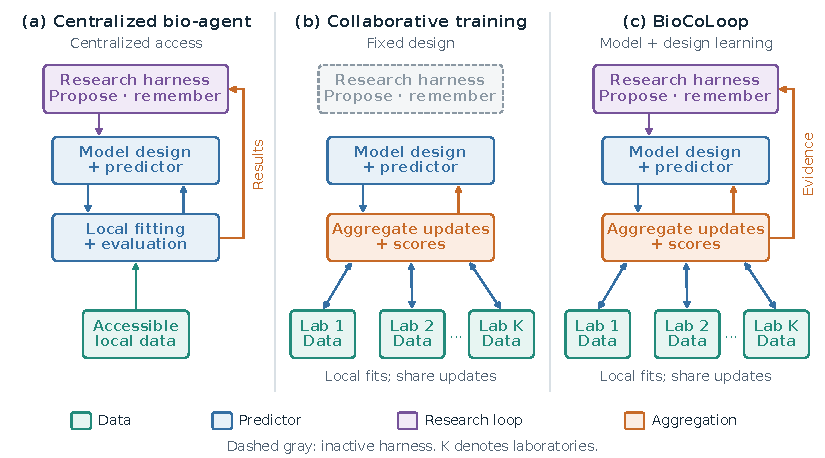
\includegraphics[width=\linewidth]{assets/paradigm_comparison.pdf}
\caption{
Research settings for biological AI.
A centralized bio-agent revises a model using centrally accessible data.
Collaborative training allows $K$ laboratories to optimize the same model and training configuration by sharing model updates rather than raw data.
BioCoLoop additionally uses results from local evaluation to guide subsequent changes to the model and training configuration.
}
\label{fig:paradigms}
\end{figure}
Our contributions are summarized as:
\begin{itemize}
\setlength{\parskip}{4pt}

\item We introduce BioCoLoop, a collaborative research framework that extends collaboration from parameter fitting to model development itself, allowing multiple laboratories to contribute without centralizing their raw data.

\item We develop a two-level procedure with an inner loop for collaborative training and evaluation and an outer loop for model development. Evaluation results from the inner loop are used to determine what model structure or training hyperparameters to test next, and which models should receive further training.

\item We validate the effectiveness of BioCoLoop on diverse scenarios, including drug--target interaction prediction, observed-response proteomic efficacy prediction, and cell perturbation identification. We further show that, with the same total amount of training and evaluation, using early evaluation results to decide which models continue training can improve performance.

\end{itemize}
